\documentclass[]{article}
\usepackage{lmodern}
\usepackage{amssymb,amsmath}
\usepackage{ifxetex,ifluatex}
\usepackage{fixltx2e} % provides \textsubscript
\ifnum 0\ifxetex 1\fi\ifluatex 1\fi=0 % if pdftex
  \usepackage[T1]{fontenc}
  \usepackage[utf8]{inputenc}
\else % if luatex or xelatex
  \ifxetex
    \usepackage{mathspec}
  \else
    \usepackage{fontspec}
  \fi
  \defaultfontfeatures{Ligatures=TeX,Scale=MatchLowercase}
\fi
% use upquote if available, for straight quotes in verbatim environments
\IfFileExists{upquote.sty}{\usepackage{upquote}}{}
% use microtype if available
\IfFileExists{microtype.sty}{%
\usepackage{microtype}
\UseMicrotypeSet[protrusion]{basicmath} % disable protrusion for tt fonts
}{}
\usepackage[margin=1in]{geometry}
\usepackage{hyperref}
\hypersetup{unicode=true,
            pdftitle={Project 1 : Test a Perceptual Phenomenon},
            pdfauthor={Isabel María Villalba Jiménez},
            pdfborder={0 0 0},
            breaklinks=true}
\urlstyle{same}  % don't use monospace font for urls
\usepackage{color}
\usepackage{fancyvrb}
\newcommand{\VerbBar}{|}
\newcommand{\VERB}{\Verb[commandchars=\\\{\}]}
\DefineVerbatimEnvironment{Highlighting}{Verbatim}{commandchars=\\\{\}}
% Add ',fontsize=\small' for more characters per line
\usepackage{framed}
\definecolor{shadecolor}{RGB}{248,248,248}
\newenvironment{Shaded}{\begin{snugshade}}{\end{snugshade}}
\newcommand{\KeywordTok}[1]{\textcolor[rgb]{0.13,0.29,0.53}{\textbf{{#1}}}}
\newcommand{\DataTypeTok}[1]{\textcolor[rgb]{0.13,0.29,0.53}{{#1}}}
\newcommand{\DecValTok}[1]{\textcolor[rgb]{0.00,0.00,0.81}{{#1}}}
\newcommand{\BaseNTok}[1]{\textcolor[rgb]{0.00,0.00,0.81}{{#1}}}
\newcommand{\FloatTok}[1]{\textcolor[rgb]{0.00,0.00,0.81}{{#1}}}
\newcommand{\ConstantTok}[1]{\textcolor[rgb]{0.00,0.00,0.00}{{#1}}}
\newcommand{\CharTok}[1]{\textcolor[rgb]{0.31,0.60,0.02}{{#1}}}
\newcommand{\SpecialCharTok}[1]{\textcolor[rgb]{0.00,0.00,0.00}{{#1}}}
\newcommand{\StringTok}[1]{\textcolor[rgb]{0.31,0.60,0.02}{{#1}}}
\newcommand{\VerbatimStringTok}[1]{\textcolor[rgb]{0.31,0.60,0.02}{{#1}}}
\newcommand{\SpecialStringTok}[1]{\textcolor[rgb]{0.31,0.60,0.02}{{#1}}}
\newcommand{\ImportTok}[1]{{#1}}
\newcommand{\CommentTok}[1]{\textcolor[rgb]{0.56,0.35,0.01}{\textit{{#1}}}}
\newcommand{\DocumentationTok}[1]{\textcolor[rgb]{0.56,0.35,0.01}{\textbf{\textit{{#1}}}}}
\newcommand{\AnnotationTok}[1]{\textcolor[rgb]{0.56,0.35,0.01}{\textbf{\textit{{#1}}}}}
\newcommand{\CommentVarTok}[1]{\textcolor[rgb]{0.56,0.35,0.01}{\textbf{\textit{{#1}}}}}
\newcommand{\OtherTok}[1]{\textcolor[rgb]{0.56,0.35,0.01}{{#1}}}
\newcommand{\FunctionTok}[1]{\textcolor[rgb]{0.00,0.00,0.00}{{#1}}}
\newcommand{\VariableTok}[1]{\textcolor[rgb]{0.00,0.00,0.00}{{#1}}}
\newcommand{\ControlFlowTok}[1]{\textcolor[rgb]{0.13,0.29,0.53}{\textbf{{#1}}}}
\newcommand{\OperatorTok}[1]{\textcolor[rgb]{0.81,0.36,0.00}{\textbf{{#1}}}}
\newcommand{\BuiltInTok}[1]{{#1}}
\newcommand{\ExtensionTok}[1]{{#1}}
\newcommand{\PreprocessorTok}[1]{\textcolor[rgb]{0.56,0.35,0.01}{\textit{{#1}}}}
\newcommand{\AttributeTok}[1]{\textcolor[rgb]{0.77,0.63,0.00}{{#1}}}
\newcommand{\RegionMarkerTok}[1]{{#1}}
\newcommand{\InformationTok}[1]{\textcolor[rgb]{0.56,0.35,0.01}{\textbf{\textit{{#1}}}}}
\newcommand{\WarningTok}[1]{\textcolor[rgb]{0.56,0.35,0.01}{\textbf{\textit{{#1}}}}}
\newcommand{\AlertTok}[1]{\textcolor[rgb]{0.94,0.16,0.16}{{#1}}}
\newcommand{\ErrorTok}[1]{\textcolor[rgb]{0.64,0.00,0.00}{\textbf{{#1}}}}
\newcommand{\NormalTok}[1]{{#1}}
\usepackage{graphicx,grffile}
\makeatletter
\def\maxwidth{\ifdim\Gin@nat@width>\linewidth\linewidth\else\Gin@nat@width\fi}
\def\maxheight{\ifdim\Gin@nat@height>\textheight\textheight\else\Gin@nat@height\fi}
\makeatother
% Scale images if necessary, so that they will not overflow the page
% margins by default, and it is still possible to overwrite the defaults
% using explicit options in \includegraphics[width, height, ...]{}
\setkeys{Gin}{width=\maxwidth,height=\maxheight,keepaspectratio}
\IfFileExists{parskip.sty}{%
\usepackage{parskip}
}{% else
\setlength{\parindent}{0pt}
\setlength{\parskip}{6pt plus 2pt minus 1pt}
}
\setlength{\emergencystretch}{3em}  % prevent overfull lines
\providecommand{\tightlist}{%
  \setlength{\itemsep}{0pt}\setlength{\parskip}{0pt}}
\setcounter{secnumdepth}{0}
% Redefines (sub)paragraphs to behave more like sections
\ifx\paragraph\undefined\else
\let\oldparagraph\paragraph
\renewcommand{\paragraph}[1]{\oldparagraph{#1}\mbox{}}
\fi
\ifx\subparagraph\undefined\else
\let\oldsubparagraph\subparagraph
\renewcommand{\subparagraph}[1]{\oldsubparagraph{#1}\mbox{}}
\fi

%%% Use protect on footnotes to avoid problems with footnotes in titles
\let\rmarkdownfootnote\footnote%
\def\footnote{\protect\rmarkdownfootnote}

%%% Change title format to be more compact
\usepackage{titling}

% Create subtitle command for use in maketitle
\newcommand{\subtitle}[1]{
  \posttitle{
    \begin{center}\large#1\end{center}
    }
}

\setlength{\droptitle}{-2em}
  \title{Project 1 : Test a Perceptual Phenomenon}
  \pretitle{\vspace{\droptitle}\centering\huge}
  \posttitle{\par}
  \author{Isabel María Villalba Jiménez}
  \preauthor{\centering\large\emph}
  \postauthor{\par}
  \predate{\centering\large\emph}
  \postdate{\par}
  \date{6 de diciembre de 2016}


\begin{document}
\maketitle

\section{Project Instructions}\label{project-instructions}

\subsection{Background Information}\label{background-information}

In a Stroop task, participants are presented with a list of words, with
each word displayed in a color of ink. The participant's task is to say
out loud the color of the ink in which the word is printed. The task has
two conditions: a congruent words condition, and an incongruent words
condition. In the congruent words condition, the words being displayed
are color words whose names match the colors in which they are printed:
for example {RED }, {BLUE }. In the incongruent words condition, the
words displayed are color words whose names do not match the colors in
which they are printed: for example {PURPLE}, { ORANGE}. In each case,
we measure the time it takes to name the ink colors in equally-sized
lists. Each participant will go through and record a time from each
condition.

\subsection{Questions For
Investigation}\label{questions-for-investigation}

As a general note, be sure to keep a record of any resources that you
use or refer to in the creation of your project. You will need to report
your sources as part of the project submission.

\subsubsection{1. What is our independent variable? What is our
dependent
variable?}\label{what-is-our-independent-variable-what-is-our-dependent-variable}

\begin{quote}
The \textbf{independent variabled} are the conditions (congruent and
incongruent), and the \textbf{dependent variable} is the time to name
the ink color in equally-sized lits.
\end{quote}

\subsubsection{2. What is an appropriate set of hypotheses for this
task? What kind of statistical test do you expect to perform? Justify
your
choices.}\label{what-is-an-appropriate-set-of-hypotheses-for-this-task-what-kind-of-statistical-test-do-you-expect-to-perform-justify-your-choices.}

\begin{quote}
The null hypothesis will be that congruent's and incongruent's condition
times will be the same, that people will identify equally fast the color
in both conditions. The alternative hypothesis will be that the mean is
changed.
\end{quote}

\begin{quote}
I expect to perform a \textbf{single-tailed test} , since I think the
time for the \emph{incongruent} case will be higher than the one for the
\emph{congruent} case. Details of the means will be reviewed in the next
section. One option can be to perform the test on \textbf{differential
measures} to check the variations.
\end{quote}

\begin{quote}
Hence, the hypotheses will be:
\end{quote}

\begin{quote}
\begin{itemize}
\tightlist
\item
  \(H_0 : \mu_{c} = \mu_{i} \rightarrow \mu_D =0\)
\item
  \(H_a : \mu_{c} \neq \mu_{i} \rightarrow \mu_D \neq 0\)
\end{itemize}
\end{quote}

\begin{quote}
for \emph{c} and \emph{i} standing, respectively, for \emph{congruent}
and \emph{incongruent}.
\end{quote}

Now it's your chance to try out the Stroop task for yourself. Go to this
\href{https://faculty.washington.edu/chudler/java/ready.html}{link},
which has a Java-based applet for performing the Stroop task. Record the
times that you received on the task (you do not need to submit your
times to the site.) Now, download this
\href{https://drive.google.com/file/d/0B9Yf01UaIbUgQXpYb2NhZ29yX1U/view?usp=sharing}{dataset}
which contains results from a number of participants in the task. Each
row of the dataset contains the performance for one participant, with
the first number their results on the congruent task and the second
number their performance on the incongruent task.

\subsubsection{3. Report some descriptive statistics regarding this
dataset. Include at least one measure of central tendency and at least
one measure of
variability.}\label{report-some-descriptive-statistics-regarding-this-dataset.-include-at-least-one-measure-of-central-tendency-and-at-least-one-measure-of-variability.}

\begin{Shaded}
\begin{Highlighting}[]
\KeywordTok{library}\NormalTok{(reshape2)}
\NormalTok{df <-}\StringTok{ }\KeywordTok{read.csv}\NormalTok{(}\StringTok{"~/Git/data-analyst-nanodegree/P1/stroopdata.csv"}\NormalTok{, }
    \DataTypeTok{sep =} \StringTok{","}\NormalTok{, }\DataTypeTok{header =} \OtherTok{TRUE}\NormalTok{)}

\CommentTok{# Total population}
\NormalTok{mu_total <-}\StringTok{ }\KeywordTok{mean}\NormalTok{(}\KeywordTok{melt}\NormalTok{(df)$value)}
\NormalTok{s_total <-}\StringTok{ }\KeywordTok{sd}\NormalTok{(}\KeywordTok{melt}\NormalTok{(df)$value)}
\KeywordTok{sprintf}\NormalTok{(}\StringTok{"Total mean is %.3f s, standard deviation is %.3f s"}\NormalTok{, }
    \NormalTok{mu_total, s_total)}

\CommentTok{# Differential case}
\NormalTok{df.diff <-}\StringTok{ }\NormalTok{df$Incongruent -}\StringTok{ }\NormalTok{df$Congruent}

\NormalTok{mu_diff <-}\StringTok{ }\KeywordTok{mean}\NormalTok{(df.diff)}
\NormalTok{s_diff <-}\StringTok{ }\KeywordTok{sqrt}\NormalTok{(}\KeywordTok{sum}\NormalTok{((df.diff -}\StringTok{ }\NormalTok{mu_diff)^}\DecValTok{2}\NormalTok{)/(}\KeywordTok{length}\NormalTok{(df.diff) -}\StringTok{ }
\StringTok{    }\DecValTok{1}\NormalTok{))}
\KeywordTok{sprintf}\NormalTok{(}\StringTok{"Mean of differences is %.3f s, standard deviation is %.3f s"}\NormalTok{, }
    \NormalTok{mu_diff, s_diff)}

\CommentTok{# Congruent}
\NormalTok{mu_c <-}\StringTok{ }\KeywordTok{mean}\NormalTok{(df$Congruent)}
\NormalTok{s_c <-}\StringTok{ }\KeywordTok{sd}\NormalTok{(df$Congruent)}

\KeywordTok{sprintf}\NormalTok{(}\StringTok{"Congruent mean is %.3f s, standard deviation is %.3f s"}\NormalTok{, }
    \NormalTok{mu_c, s_c)}

\CommentTok{# Inconruent}
\NormalTok{mu_i <-}\StringTok{ }\KeywordTok{mean}\NormalTok{(df$Incongruent)}
\NormalTok{s_i <-}\StringTok{ }\KeywordTok{sd}\NormalTok{(df$Incongruent)}

\KeywordTok{sprintf}\NormalTok{(}\StringTok{"Incogruent mean is %.3f s, standard deviation is %.3f s"}\NormalTok{, }
    \NormalTok{mu_i, s_i)}
\end{Highlighting}
\end{Shaded}

\begin{quote}
The mean for the \textbf{congruent condition} is 14.051 s with a
standard deviation of 3.559 s.
\end{quote}

\begin{quote}
The mean for the \textbf{incongruent condition} is 22.016 s with a
standard deviation of 4.797 s.
\end{quote}

\begin{quote}
The mean of the \textbf{difference} is 7.965 s with a standard deviation
of 4.865 s.
\end{quote}

\subsubsection{4. Provide one or two visualizations that show the
distribution of the sample data. Write one or two sentences noting what
you observe about the plot or
plots.}\label{provide-one-or-two-visualizations-that-show-the-distribution-of-the-sample-data.-write-one-or-two-sentences-noting-what-you-observe-about-the-plot-or-plots.}

\begin{Shaded}
\begin{Highlighting}[]
\KeywordTok{library}\NormalTok{(ggplot2)}
\KeywordTok{library}\NormalTok{(reshape2)}

\KeywordTok{library}\NormalTok{(plyr)}
\NormalTok{mu <-}\StringTok{ }\KeywordTok{ddply}\NormalTok{(}\KeywordTok{melt}\NormalTok{(df), }\StringTok{"variable"}\NormalTok{, summarise, }\DataTypeTok{grp.mean =} \KeywordTok{mean}\NormalTok{(value))}

\NormalTok{p <-}\StringTok{ }\KeywordTok{ggplot}\NormalTok{(}\KeywordTok{melt}\NormalTok{(df), }\KeywordTok{aes}\NormalTok{(}\DataTypeTok{x =} \NormalTok{value, }\DataTypeTok{fill =} \NormalTok{variable)) +}\StringTok{ }
\StringTok{    }\KeywordTok{geom_histogram}\NormalTok{(}\KeywordTok{aes}\NormalTok{(}\DataTypeTok{y =} \NormalTok{..density..), }\DataTypeTok{alpha =} \FloatTok{0.3}\NormalTok{) +}\StringTok{ }
\StringTok{    }\KeywordTok{geom_density}\NormalTok{(}\KeywordTok{aes}\NormalTok{(}\DataTypeTok{x =} \NormalTok{value, }\DataTypeTok{color =} \NormalTok{variable), }\DataTypeTok{alpha =} \FloatTok{0.6}\NormalTok{, }
        \DataTypeTok{linetype =} \StringTok{"dashed"}\NormalTok{)}

\CommentTok{# Add mean lines}
\NormalTok{p +}\StringTok{ }\KeywordTok{geom_vline}\NormalTok{(}\DataTypeTok{data =} \NormalTok{mu, }\KeywordTok{aes}\NormalTok{(}\DataTypeTok{xintercept =} \NormalTok{grp.mean, }\DataTypeTok{color =} \NormalTok{variable), }
    \DataTypeTok{linetype =} \StringTok{"dashed"}\NormalTok{, }\DataTypeTok{alpha =} \DecValTok{1}\NormalTok{)}
\end{Highlighting}
\end{Shaded}

\begin{figure}[htbp]
\centering
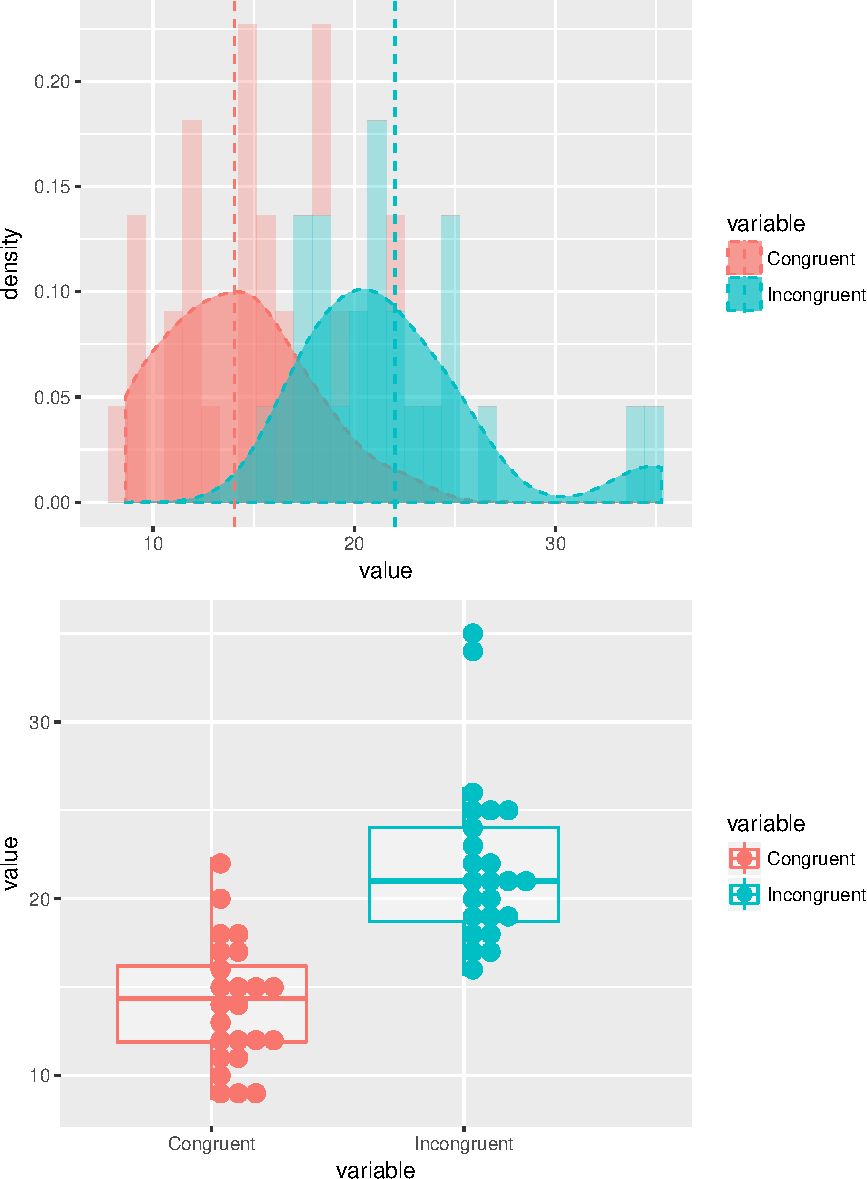
\includegraphics{P1-Test_a_Perceptual_Phenomenon_files/figure-latex/visualization-1.pdf}
\caption{Data distribution \label{fig1_normal}}
\end{figure}

\begin{quote}
Both the \emph{congruent} and the \emph{incongruent} group are normal
distributions with different mean values (bigger mean time for the
\emph{incongruent} case) and similar standard deviations. In the case of
the incongruent condition there is a significant presence of outlieres
in the upper side of the distribution.
\end{quote}

\subsubsection{5. Now, perform the statistical test and report your
results. What is your confidence level and your critical statistic
value? Do you reject the null hypothesis or fail to reject it? Come to a
conclusion in terms of the experiment task. Did the results match up
with your
expectations?}\label{now-perform-the-statistical-test-and-report-your-results.-what-is-your-confidence-level-and-your-critical-statistic-value-do-you-reject-the-null-hypothesis-or-fail-to-reject-it-come-to-a-conclusion-in-terms-of-the-experiment-task.-did-the-results-match-up-with-your-expectations}

\begin{Shaded}
\begin{Highlighting}[]
\NormalTok{df_diff <-}\StringTok{ }\KeywordTok{data.frame}\NormalTok{(df.diff)}
\NormalTok{n <-}\StringTok{ }\KeywordTok{nrow}\NormalTok{(df_diff)}
\NormalTok{dfr <-}\StringTok{ }\NormalTok{n -}\StringTok{ }\DecValTok{1}
\NormalTok{SE <-}\StringTok{ }\NormalTok{s_diff/}\KeywordTok{sqrt}\NormalTok{(n)}
\NormalTok{t <-}\StringTok{ }\NormalTok{mu_diff/SE}
\end{Highlighting}
\end{Shaded}

\paragraph{\texorpdfstring{\textbf{Hypotheses}}{Hypotheses}}\label{hypotheses}

\begin{quote}
\begin{itemize}
\tightlist
\item
  \(H_0 : \mu_{c} = \mu_{i} \rightarrow \mu_D =0\)
\item
  \(H_a : \mu_{c} \neq \mu_{i} \rightarrow \mu_D \neq 0\)
\end{itemize}
\end{quote}

\paragraph{\texorpdfstring{\textbf{Difference
test}}{Difference test}}\label{difference-test}

\begin{quote}
The test used is the difference test, which is used to evaluate the
performance on a group of subjects after changing the conditions, as it
is done in the Stroop experiment. The steps are the following (Shier
2014, Cognitive Science (n.d.)):
\end{quote}

\begin{quote}
\begin{enumerate}
\def\labelenumi{\arabic{enumi}.}
\tightlist
\item
  Calculate the difference \(d= t_i-t_c\)
\item
  Calculate the mean of the difference \(\bar{d}=\) 7.965 s
\item
  Calculate the standard error \(SE(\bar{d})= \frac{s_d}{\sqrt{n}}\),
  for \(s_d\) the standard deviation of the differences.
  \(SE(\bar{d})= \frac{s_d}{\sqrt{n}}=\) 0.993 s
\item
  Calculate the t-statistic: \(t=\frac{\bar{d}}{SE(\bar{d})}=\) 8.021.
  Under the null distribution this statistic follows a t-distribution
  with n-1 (23) degrees of freedom.
\item
  See where t falls in the \(t_{n-1}\) distribution Get the value fron
  the table: this will give the p-value for the paired t-test (Udacity,
  n.d.). \(t_{critical}=\) 1.714
\end{enumerate}
\end{quote}

\begin{quote}
\(t> t_{critical} \rightarrow\) t lies in the critical region
\end{quote}

\begin{quote}
\textbf{ Results are statistically significant: NULL is REJECTED }
\end{quote}

\paragraph{\texorpdfstring{\textbf{Margin of
error}}{Margin of error}}\label{margin-of-error}

\begin{quote}
\(\bar{d} \pm t^* \frac{s_d}{\sqrt{n}}=\) {[}5.911s, 10.019s{]} for
\(t^*\) the value for 2.5\% fot a t-distribution for n-1 degrees of
freedom.
\end{quote}

\paragraph{\texorpdfstring{\textbf{Cohen's
d}}{Cohen's d}}\label{cohens-d}

\begin{quote}
For the case of the paired test, Cohen's d is defined as the difference
of means between the post-test and pre-test treatments divided by the
standard deviation of the pre-test condition.
\end{quote}

\begin{quote}
\(Cohen's\; d= \frac{\mu_i-\mu_c}{SD_c}=\) 2.238
\end{quote}

\paragraph{\texorpdfstring{\textbf{Coefficient of determination
\(r^2\)}}{Coefficient of determination r\^{}2}}\label{coefficient-of-determination-r2}

\begin{quote}
\(r^2= \frac{t^2}{t^2+df}=\) 0.737
\end{quote}

\subsubsection{6. Optional: What do you think is responsible for the
effects observed? Can you think of an alternative or similar task that
would result in a similar effect? Some research about the problem will
be helpful for thinking about these two
questions!}\label{optional-what-do-you-think-is-responsible-for-the-effects-observed-can-you-think-of-an-alternative-or-similar-task-that-would-result-in-a-similar-effect-some-research-about-the-problem-will-be-helpful-for-thinking-about-these-two-questions}

\begin{quote}
The changes are produced by applying a different treatment to the same
users. Hence, their response will be altered, A similar effect could be
observed in when retrieveing the performance of students before and
after studying.
\end{quote}

\section*{References}\label{references}
\addcontentsline{toc}{section}{References}

\hypertarget{refs}{}
\hypertarget{ref-slides_t_test}{}
Cognitive Science, Department of. n.d. BME Faculty of Natural Sciences
of Budapest.
\url{http://www.cogsci.bme.hu/~ktkuser/KURZUSOK/BMETE47MC38/2015_2016_1/7_The\%}.

\hypertarget{ref-stanford_t_test}{}
Shier, Rosoe. 2014. ``Paired T-Tests.'' online.
\url{http://www.statstutor.ac.uk/resources/uploaded/paired-t-test.pdf}.

\hypertarget{ref-t-table}{}
Udacity. n.d. ``T-Table.''
\url{https://s3.amazonaws.com/udacity-hosted-downloads/t-table.jpg}.


\end{document}
